%% Template para dissertação/tese na classe UFPEthesis
%% versão 0.9.2
%% (c) 2005 Paulo G. S. Fonseca
%% www.cin.ufpe.br/~paguso/ufpethesis

%% Carrega a classe ufpethesis
%% Opções: * Idiomas
%%           pt   - português (padrão)
%%           en   - inglês
%%         * Tipo do Texto
%%           bsc  - para monografias de graduação
%%           msc  - para dissertações de mestrado (padrão)
%%           qual - exame de qualificação doutorado
%%           prop - proposta de tese doutorado
%%           phd  - para teses de doutorado
%%         * Mídia
%%           scr  - para versão eletrônica (PDF) / consulte o guia do usuario
%%         * Estilo
%%           classic - estilo original à la TAOCP
%%           modern  - estilo à la CUP (padrão)
%%           ugly    - formato da UFPE com parte pré-textual no formato ABNT
%%         * Paginação
%%           oneside - para impressão em face única
%%           twoside - para impressão em frente e verso (padrão)
\documentclass{ufpethesis}
% Paquetes LaTeX y estilos globales
%\usepackage[utf8]{inputenc}
%\usepackage[portugues,english]{babel}
%\usepackage[portuguese,english]{babel}
\usepackage{multicol}
\usepackage{xcolor}
\usepackage{subfigure}
%\usepackage[spanish]{babel}

\usepackage{graphicx}
%\usepackage{color}% para colocar la tabla
\usepackage{graphicx}
%\usepackage{float}
\usepackage{titlesec}
\usepackage[bookmarks,breaklinks,colorlinks=true,allcolors=black, citecolor=blue]{hyperref}
%\usepackage[hidelinks,colorlinks=true,linkcolor=blue,citecolor=blue]{hyperref}
\usepackage{listings}
\usepackage{inconsolata}
\usepackage{float}

%\usepackage[square,numbers]{natbib}
%\AtBeginDocument{
%  \renewcommand{\bibsection}{\chapter{\bibname}}
%} % Bibliografia en capitulo numerado

%\usepackage{geometry}
\usepackage{amsmath,amsthm}% cambia la fuente de la letra y ecuaciones con amsfonts,
%\usepackage{amsmath}  % For math
\usepackage{amssymb}  % For more math

\usepackage{parskip}
%\usepackage[official]{eurosym}
\usepackage{todonotes}
\usepackage{csquotes}

% new fuente
\usepackage{tgtermes}
\usepackage{float}
\usepackage{bm}
\usepackage{graphicx} % Required for including pictures
\usepackage{mathtools}
%\usepackage{multicol}
%\usepackage{caption} % For caption spacing
%\usepackage{subcaption} % For sub-figures

\usepackage{booktabs} % better tables
\usepackage{rotating} % landscape stuff, such as tables
\usepackage{array} % for m columns
\usepackage{multirow} % multi row tables
%\usepackage{bigdelim} % for big braces in tables (https://tex.stackexchange.com/a/129797/66561)

%\usepackage{afterpage} % for using \afterpage{\clearpage} before sidewaysfigures, to prevent them from going to the end:
%https://latex.org/forum/viewtopic.php?t=5903

%\usepackage[skip=-2pt, position=top, labelfont=normalfont]{subcaption} % multiple figures in one
%skip=-2pt reduces space between caption and subfigure
%singlelinecheck=false, justification=raggedright move the caption to the left

%\usepackage{microtype}%micro-typographic extension for better looks (subliminal refinements towards typographical perfection)
%%\usepackage{textcomp}% Solves some warnings....
%\usepackage[titletoc, title, header]{appendix}% For nicer appendices

%\usepackage{tabularx} % better tables

%\usepackage{multicol} % itemizations on multiple columns

%\newcommand{\HRule}{\rule{.9\linewidth}{.6pt}} % New command to make the lines in the title page
\newcommand{\decoRule}{\rule{.8\textwidth}{.4pt}} % New command for a rule to be used under figures
%\newcommand{\halfDecoRule}{\rule{.4\textwidth}{.4pt}} % New command for a rule to be used under figures

% con el comando \par empieza un nuevo parrafo con sangria, y con \\ comienza una nueva línea pero no un nuevo párrafo.
% las subsecciones empiezan sin sangria \parindent \indent
%\noindent to remove
% se establecerá en cero cuando se inserte un encabezado de sección
%\usepackage{indentfirst}
%set title spacing
%\usepackage{indentfirst}

\setlength\parindent{24pt}
\setlength{\parskip}{3.0pt}
\titlespacing*{\section}{0pt}{3.5ex plus 1ex minus .2ex}{2.3ex plus .2ex}
\titlespacing*{\subsection}{0pt}{3.5ex plus 1ex minus .2ex}{2.3ex plus .2ex}
%\usepackage{parskip}
%\setstretch{1.20}

% fancy chapter
\usepackage[Lenny]{fncychap}

%\usepackage{enumitem}%abreviaciones
%	HEADERS AND FOOTERS
%----------------------------------------------------------------------------------------
% abbreviations
%	ABBREVIATIONS PAGE DESIGN
%----------------------------------------------------------------------------------------
%--------------------------References
 %\usepackage[backend=biber, style=numeric, citestyle=nature]{biblatex}
 
% \usepackage{csquotes}
 % \usepackage[babel]{csquotes}
%\usepackage[style=numeric, maxbibnames=99, giveninits]{biblatex}

 % giveninits : es para colocar solo la inicial del nombre
 % giveninits : es para colocar solo la inicial del nombre

\usepackage[style=numeric-comp, sorting=none, backend=bibtex, doi=false, isbn=false, natbib=true, giveninits]{biblatex} % sorting=none ordena por orden de citas

\addbibresource{references.bib}

%\setlength\bibitemsep{5\itemsep}
\setlength{\bibitemsep}{\parskip}% para colocar espacio entre los items de referencias

% para colocar la tabla de revision bibliografica
%\usepackage{osameet3}
\usepackage{booktabs, longtable,array}
\usepackage{color, colortbl}
%\definecolor{name}{system}{definition}
\definecolor{Gray}{gray}{0.9}
%\usepackage[table]{xcolor}
\newcolumntype{P}[1]{>{\raggedright\arraybackslash}p{#1}}
%\input{etc/style}

%% Preâmbulo:
%% coloque aqui o seu preâmbulo LaTeX, i.e., declaração de pacotes,
%% (re)definições de macros, medidas, etc.

%% Identificação:

% Universidade
% e.g. \university{Universidade de Campinas}
% Na UFPE, comente a linha a seguir
\university{Universidade Federal de Pernambuco}

% Modifique o comando \universitylogo para alterar o logo da universidade
% e.g.
% \renewcommand{\universitylogo}{\includegraphics{newlogo.pdf}}

% Endereço (cidade)
% e.g. \address{Campinas}
% Na UFPE, comente a linha a seguir
\address{Recife}

% Instituto ou Centro Acadêmico
% e.g. \institute{Centro de Ciências Exatas e da Natureza}
% Comente se não se aplicar
\institute{Centro de Ciências Exatas e da Natureza}

% Departamento acadêmico
% e.g. \department{Departamento de Informática}
% Comente se não se aplicar
%\department{Programa de
%Pós-graduação em Estatística}

 

% e.g. \program{Pós-graduação em Ciência da Computação}
\program{Pós-graduação em Estatística}

% Área de titulação
% e.g. \majorfield{Ciência da Computação}
%\majorfield{Programa de
%Pós-graduação em Estatística}

% Título da dissertação/tese
% e.g. \title{Sobre a conjectura $P=NP$}
\title{Fusão Explicável de Evidências Estatísticas de Bordas em Imagens}

% Data da defesa
% e.g. \date{19 de fevereiro de 2003}
\date{2022}

% Autor
% e.g. \author{José da Silva}
\author{Rosa Janeth Alpala}

% Orientador(a)
% Opção: [f] - para orientador do sexo feminino
% e.g. \adviser[f]{Profa. Dra. Maria Santos}
\adviser{Dr. Alejandro C. Frery}

% Orientador(a)
% Opção: [f] - para orientador do sexo feminino
% e.g. \coadviser{Prof. Dr. Pedro Pedreira}
% Comente se não se aplicar
%\coadviser{NOME DO(DA) CO-ORIENTADOR(A)}

%% Inicio do documento

%\setlength\headheight{15pt}

%colocar linea en la cabecera
%\usepackage{fancyhdr}
%\fancyhf{}
%\fancyhead[CE]{\small\slshape\leftmark}
%\fancyhead[CO]{\small\slshape\rightmark}
%\fancyfoot[CE,CO]{\small\thepage}
%\renewcommand{\headrulewidth}{0.4pt}
%\renewcommand{\footrulewidth}{0.4pt}


%\pagestyle{fancy} %coloca la linea en la cabecera


\begin{document}

%%
%% Parte pré-textual
%%

\frontmatter
% Folha de rosto
% Comente para ocultar
\frontpage

% Portada (apresentação)
% Comente para ocultar
%\pagestyle{empty}
%\pagenumbering{gobble}
%\pagenumbering{alph}
%\thispagestyle{empty}
\cleardoublepage
    %Abstract - begin
        \begingroup
        \let\clearpage\relax
        \let\cleardoublepage\relax
        \let\cleardoublepage\relax

\presentationpage %<======= subportada
\thispagestyle{empty}%<=======
        \endgroup           
        \vfill 
\newpage
%\thispagestyle{empty}
%\frontmatter
%\cleardoublepage% \clearpage
%\pagenumbering{roman}

% Dedicatória
% Comente para ocultar
%\begin{dedicatory}
%DIGITE A DEDICATÓRIA AQUI
%\end{dedicatory}

% Agradecimentos
% Se preferir, crie um arquivo à parte e o inclua via \include{}
%\acknowledgements
%DIGITE OS AGRADECIMENTOS AQUI

% Epígrafe
% Comente para ocultar
% e.g.
%  \begin{epigraph}[Tarde, 1919]{Olavo Bilac}
%  Última flor do Lácio, inculta e bela,\\
%  És, a um tempo, esplendor e sepultura;\\
%  Ouro nativo, que, na ganga impura,\\
%  A bruta mina entre os cascalhos vela.
%  \end{epigraph}
%\begin{epigraph}[NOTA]{AUTOR}
%DIGITE AQUI A CITAÇÃO
%\end{epigraph}

% Resumo em Português
% Se preferir, crie um arquivo à parte e o inclua via \include{}
%\resumo
%DIGITE O RESUMO AQUI
% Palavras-chave do resumo em Português
%\begin{keywords}
%DIGITE AS PALAVRAS-CHAVE AQUI
%\end{keywords}

% Resumo em Inglês
% Se preferir, crie um arquivo à parte e o inclua via \include{}

%\newpage
%\pagenumbering{arabic}

\setcounter{page}{2}
%\pagestyle{plain}
%
%\begin{otherlanguage}{spanish}
\begin{abstract}
\phantomsection
\addcontentsline{toc}{chapter}{Abstract}
%\addchaptertocentry{\abstrname}
%\addchaptertocentry{\abstractname} % Add the abstract to the table of contents
Edge detection has an essential role in post-processing of Polarimetric synthetic aperture radar (PolSAR) images. It is still a big challenge to extract all the edge features and suppress speckle noises, especially when weak/strong edges appear simultaneously inside and outside heterogeneous areas.

PolSAR images can provide more information than single-polarimetric synthetic aperture radar (SAR) images. As the prerequisite step of image processing, PolSAR edge detection is very important, which can provide important structural information for further object recognition and image interpretation of PolSAR images. However, a complex PolSAR scene usually includes both heterogenous and homogenous terrain types such as urban areas, forests, farmlands, waters, and so on.

In this thesis, we obtain the statistical properties (bias, variance) of edge point estimators in SAR/PolSAR images. In this way, we propose and evaluate new fusion and evidence selection techniques that take these properties into account.

\end{abstract}
%\end{otherlanguage}
%\addcontentsline{toc}{chapter}{Abstract}
%\addcontentsline{toc}{chapter}{\protect\numberline{\abstrname}}
\clearpage

%\addcontentsline{toc}{section}{abstract}
%\abstract
\newpage
\begin{otherlanguage}{portuguese} 


\begin{resumo}
\phantomsection
\addcontentsline{toc}{chapter}{Resumo}
%\addchaptertocentry{\resumenname} % Add the abstract to the table of contents
A detecção de bordas tem um papel essencial no pós-processamento das imagens PolSAR. A extração de todas as características das bordas e a supressão de ruídos speckle, especialmente quando bordas fracas/fortes aparecem simultaneamente dentro e fora de áreas heterogêneas, ainda é um grande desafio.

As imagens PolSAR podem fornecer mais informações do que as imagens de radar de abertura sintética (SAR) de polarimetria única. Como a etapa de pré-requisito do processamento de imagem, a detecção de bordas PolSAR é muito importante, o que pode fornecer informações estruturais importantes para reconhecimento adicional de objetos e interpretação de imagens PolSAR. No entanto, uma cena PolSAR complexa geralmente inclui tipos de terreno heterogêneos e homogêneos, como áreas urbanas, florestas, terras agrícolas, águas e assim por diante.

Nesta tese, obtemos as propriedades estatísticas (bias, variância) dos estimadores de pontos de borda em imagens SAR/PolSAR. Desta forma, propomos e avaliamos novas técnicas de fusão e seleção de evidências que levem em consideração essas propriedades.

\end{resumo}
\end{otherlanguage}
%\addcontentsline{toc}{chapter}{Resumo}
%\addcontentsline{toc}{chapter}{\protect\numberline{\resumoname}}
\clearpage
\newpage
% Palavras-chave do resumo em Inglês
%\begin{keywords}
%DIGITE AS PALAVRAS-CHAVE AQUI
%\end{keywords}

% Sumário
% Comente para ocultar
\tableofcontents

%\cleardoublepage
%\setcounter{page}{-1}
%\newpage
% Lista de figuras
% Comente para ocultar
%\listoffigures
%\newpage
% Lista de tabelas
% Comente para ocultar
%\listoftables
\newpage



%%
%% Parte textual
%%
\mainmatter
%\pagestyle{thesis} % Return the page headers back to the "thesis" style
% É aconselhável criar cada capítulo em um arquivo à parte, digamos
% "capitulo1.tex", "capitulo2.tex", ... "capituloN.tex" e depois
% incluí-los com:
% \include{capitulo1}
% \include{capitulo2}
% ...
% \include{capituloN}
%\cleardoubleemptypage
%\newpage
%\pagenumbering{arabic}


%\setcounter{page}{1}
\chapter{Introduction}\label{chp:int}
%------------------------------------
%	INTRO INTRO
%------------------------------------

The use of Statistical Information Theory (SIT) and Statistical Information Geometry (SIG) in image processing and analysis problems has the potential to provide several solutions to the same problem. Considering that these solutions are evidences, or estimates of the solution, this project aims to propose techniques for fusing them into a single solution potentially better than the individual evidences.

The starting point is the paper by de Borba et al. \cite{de2020fusion}, in which the authors obtain several evidences of the location of edge points in images with low signal/noise relation. In this work, the estimations are treated deterministically, that is, without taking into account the variability of the estimator that produces them. These estimations go through fusion processes to obtain an edge point that summarizes the evidence.

The project proposes to create fusion techniques that take into account the quality of each evidence. In this way, evidence that is subject to high variability, or that is inconsistent with most other evidence, will have less influence on the final result.

On the one hand, the project is challenging because there are no theoretical results to assess the quality (bias, variance, etc.) of the evidence. On the other hand, when they come from an analysis based on the SIT/GIS approach, there is the possibility of advancing the frontier of knowledge since there is a powerful statistical tool (although little explored) for this purpose.

An explainable fusion of this type of evidence will be able to provide semantically valuable information on the contribution of each component to the composition of the final result. With this, end-users will be able to extract relevant information about the information content (and reliability) of each source of evidence. This knowledge will allow, for example, discarding unreliable sources, or those that, being redundant, contribute little to the quality of the product.

The work will focus on SAR/PolSAR (Synthetic Aperture Radar/Polarimetric SAR) images. These images are of great relevance in Remote Sensing \cite{cloude2009polarisation}, and present high levels of non-Gaussian and non-additive noise. This last feature makes them attractive and challenging for the development of new techniques \cite{lee2017polarimetric}.

The statistical approach to edge detection in SAR/PolSAR images has provided comparable or better results than techniques previously considered state-of-the-art. Among the edge detection results to be highlighted for SAR images (in which each pixel has a non-negative value), we mention the works of \cite{gambini2008accuracy, giron2012nonparametric}.


\section{Literature Review}
A. Fink \cite{fink2019conducting} provides the following definition: ``A literature review is a systematic, explicit, and reproducible project to identify, evaluate, and interpret the existing body of recorded documents.''  Literature reviews generally aim at two goals: first, they summarize existing research by identifying patterns, themes, and issues. Second, this helps identify the conceptual content of the field and can contribute to theory development.

\subsection{Search Strategy}

In order to select the most relevant articles for this study, we started by searching for papers on edge detection in SAR/PolSAR images in the most common scientific databases: Scopus, Web of Science (WoS), Science Direct (SD), Google Scholar (GS), Emerald insight (Emerald), Wiley Online Library (Wiley), Taylor \& Francis Online (T\&F), Springer Link (Springer), Inderscience (IS), and Informs PubsOnline (IPO). \\ %The Search Terms employed in the field of Title are the following:
The employed keywords were the following focused on the fields Title-Abstract-Keywords:
\begin{itemize}
	\item ("bias correction" OR "improve estimators" OR "new estimator" OR "MLE" OR "efficient estimators" OR "maximum-likelihood estimation" OR "statistical information theory")  
\item	AND ("boundary detection" OR "edge detection" OR "edge detection method" OR "edge detector") 
\item ("PolSAR images" OR "Polarimetric Synthetic Aperture Radar" OR "single-polarimetric synthetic aperture radar images" OR "SAR images")
\end{itemize}
Some works related to this topic can be seen in Table \ref{tab:1}.
\begin{longtable}{P{\dimexpr0.26\textwidth-2\tabcolsep-2\arrayrulewidth\relax}
                        P{\dimexpr0.39\textwidth-2\tabcolsep-\arrayrulewidth\relax}
                        P{\dimexpr0.30\textwidth-2\tabcolsep-\arrayrulewidth\relax}
                        %P{\dimexpr0.20\textwidth-2\tabcolsep-\arrayrulewidth\relax}
                        }
\toprule
Author & Title & Source \\\midrule
\rowcolor{Gray}\multicolumn{3}{c}{Edge detection}\\
Nascimento, A. D., Horta, M. M., Frery, A. C., and Cintra, R. J. (2013)\cite{nascimento2013comparing}. & Comparing edge detection methods based on stochastic entropies and distances for PolSAR imagery & IEEE journal of selected topics in applied earth observations and remote sensing\\ \midrule
%\rowcolor{gray!20}\multicolumn{3}{c}{Music}\\
Xiang, Y., Wang, F., Wan, L., and You, H. (2017) \cite{xiang2017sar} & SAR-PC: Edge detection in SAR images via an advanced phase congruency model. & Remote Sensing\\ \midrule

Qin, X., Hu, T., Yu, W., Wang, P., Li, J.,  Zou, H. (2018) \cite{qin2018edge}& Edge detection of PolSAR images using statistical distance between automatically refined samples.& IEEE International Geoscience and Remote Sensing Symposium\\
\bottomrule
Nascimento, A. D., Frery, A. C.,  Cintra, R. J. (2019) \cite{nascimento2018detecting}& Detecting changes in fully polarimetric SAR imagery with statistical information theory.& IEEE Transactions on Geoscience and Remote Sensing\\
\bottomrule
Quan, S., Xiang, D., Xiong, B.,  Kuang, G. (2020) \cite{quan2019edge}& Edge detection for PolSAR images integrating scattering characteristics and optimal contrast.& IEEE Geoscience and Remote Sensing Letters\\
\bottomrule
\caption[Papers related to edge detection]{Papers related to edge detection}\label{tab:1}
%\caption{\label{Pesquisa de documentos.} works that use Machine Learning}
\end{longtable}




%("REVIEW" OR "STATE OF THE ART" OR "SURVEY" OR "CONCEPTUAL FRAMEWORK" ) AND ("LAYOUT DESIGN" OR "DESIGN OF LAYOUT" OR "MANUFACTURING LAYOUT"
%OR "FACILITY LAYOUT" OR "PLANT LAYOUT" OR "FACILITY LAYOUT PLANNING" ). 

%---------------------------------------------------------------------------------------------------------------------
\section{Project objectives}
The objective of this thesis is to contribute to the state of the art in the fusion of evidence using a statistical approach to achieve explainable and relevant results. \\

The main specific objectives are:

\begin{itemize}
	\item Obtain the statistical properties (bias, variance) of edge point estimators in SAR/PolSAR images.
	\item Propose and evaluate new fusion and evidence selection techniques that take these properties into account.
	\item Develop new features for production software, e.g. PolSARpro and SNAP.
\end{itemize}

\section{Thesis organization}\label{sec:research_questions}

% colocar para citar los capitulos
\hypersetup{linkcolor=blue}

This thesis is structured in 5 chapters. In the upcoming sections of the current chapter a general overview on ... \\
 Chapter~\ref{chp:obs} details ...\\
Chapter ~\ref{chp:models} explains ...
%------------------------------------
%	HAZARD: OVERVIEW
%------------------------------------


\section{Computing platforms}
This  project required a vast amount of computing, preprocessing, analysis and plotting.

%------------------------------------
%	TODO STUFF
%------------------------------------
% \section{Additional sources to integrate in this chapter}
% \begin{itemize}
% \item check all TODOs
% \item read again \url{http://ec.europa.eu/environment/water/flood_risk/flood_atlas/pdf/handbook_goodpractice.pdf}
% \item include citation EU Floods Directive (2007/60/EC) , \cite{Mysiak2013, EUFD2007}
% \item section to talk about uncertainties? \citet{alfieri2014} has a good section about it
% \item Alps are the water tower of the Po plain, and for this reason I might want to give them a closer look. I could cite one of the many kotlarski works, or e.g. \citet[][]{Gobiet2014}. View the 'Alps' category in my Mendeley, it contains about 30 works on the subject
% \end{itemize}
\chapter{SAR Polarimetry}\label{chp:obs}%\Cref{sec:pr_obs}
%The main observational data used within this thesis are of four different kinds: precipitation, discharge, 

%------------------------------------
%	PRECIPITATION OBS
%------------------------------------

\section{Electromagnetic radiation}
\section{SAR system characteristics} \label{sec:pr_obs}
%\subsection*{Phase and Polarization}
%Precipitation is probably the most difficult of all atmospheric climate variables to measure reliably, due to the huge spatio-temporal variability (especially in summer) and to the physical difficulty of setting up and maintaining a dense network of high-maintenance sensors. In our multi-model approach
\section{Polarimetry}

%\subsection*{Generating Polarimetric Parameters in SNAP}
	\begin{figure}[H]
    \centering
    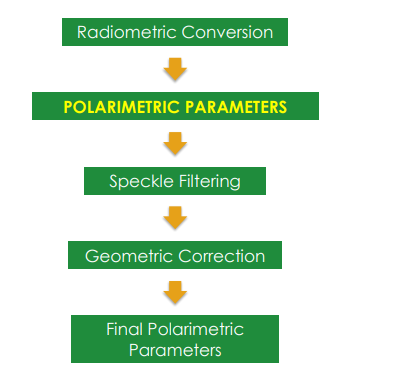
\includegraphics[width=0.4\textwidth]{figures/snap.PNG}
    \decoRule
    \caption[Generating Polarimetric Parameters in SNAP]{Generating Polarimetric Parameters in SNAP.}
    \label{fig:undercatch}
\end{figure}

	
	%\begin{wrapfigure}{l}{0.25\textwidth}
%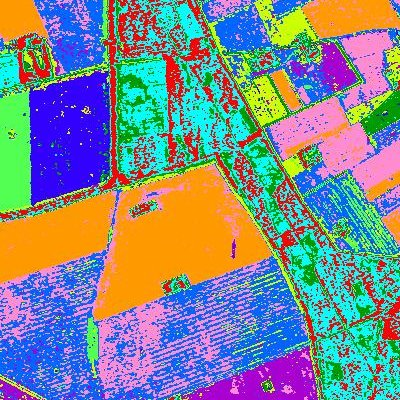
\includegraphics[width=0.9\linewidth]{figures/PolSAR.jpg}
%\caption{Ttulo 1}
%\label{F:figuranotexto}
%\end{wrapfigure}


\subsection*{Example math equations}
%-----------------------------------------------------------
%\begin{align*}
%L(\alpha,  \lambda|  \bm{x})&=\prod_{i=1}^n{f(x_i|\alpha, \lambda )}\\
                                 %&= \prod_{i=1}^n\left[\frac{\lambda^{\alpha}}{\Gamma(\alpha)}\,x_i^{\alpha-1}\exp\left\{-\lambda x_i\right\}\right]\\
%&=\left(\frac{\lambda^{\alpha}}{\Gamma(\alpha)}\right)^n\prod_{i=1}^nx_i^{\alpha-1}\times \exp\left\{-\left(\lambda\sum_{i=1}^n x_i \right)\right\}
%\end{align*}
%%----------------------------------------------------------
\begin{align}
\label{eq:em}
\ell(\alpha, \lambda| \bm{x}) &=\log\left[\left(\frac{\lambda^{\alpha}}{\Gamma(\alpha)}\right)^n\prod_{i=1}^nx_i^{\alpha-1}\times \exp\left\{-\left(\lambda\sum_{i=1}^n x_i \right)\right\}\right]\nonumber\\
&=\log\left(\frac{\lambda^{\alpha}}{\Gamma(\alpha)}\right)^n+\log\left[\prod_{i=1}^nx_i^{\alpha-1}\right]-\lambda\sum_{i=1}^nx_i\nonumber\\
&=n\log\left(\frac{\lambda^{\alpha}}{\Gamma(\alpha)}\right)+(\alpha-1)\log\prod_{i=1}^nx_i-\lambda\sum_{i=1}^nx_i\nonumber\\
&=n\log(\lambda^{\alpha})-n\log(\Gamma(\alpha))+(\alpha-1)\sum_{i=1}^n\log(x_i)-\lambda\sum_{i=1}^nx_i\nonumber\\
&=n\alpha\log \lambda -n\log(\Gamma(\alpha)) +(\alpha-1)\sum_{i=1}^n\log(x_i)-\lambda\sum_{i=1}^nx_i.
	\end{align}
%----------------------------------------------------------
\begin{figure}
    \centering
    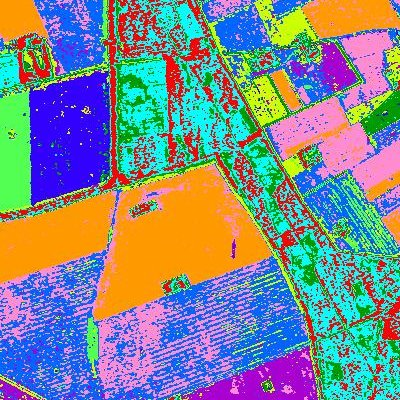
\includegraphics[width=0.5\textwidth]{figures/PolSAR.jpg}
    \decoRule
    \caption[Example plot]{Example plot.}
    \label{fig:undercatch}
\end{figure}

%-------------------------------------------------------

%\begin{table}[h]
%\centering
%\caption{\label{tab1}Comparação de tempos. }
%\begin{tabular}{l c c }
%\toprule[1pt] \textbf{Amostra (N)} \ \ \  \ \ \  & \textbf{Tempo de Execução (C)}\ \ \ \ \ \ \  &\textbf{Tempo de Execução (Ox)} \\\midrule[0.5pt]
%$20$ & 7.6810 s  &  5.01 s \\
%$30$ & 9.6260 s     & 5.34 s \\
%$50$ &  10.0310 s & 5.99 s \\
%$100$ & 15.5420 s & 8.07 s \\
%$200$ & 20.5860 s & 9.64 s \\
%$500$ & 29.0890  s & 15.12 s \\
%\bottomrule[1pt]
%\end{tabular}
%\caption[Precipitation datasets]{List of datasets used in the analysis of daily precipitation uncertainty carried over i}\label{tab:1}
%\end{table}
%------------------------------------------------------


%\begin{table}[]
%\centering
%\begin{tabular}{@{}llll@{}}
%\toprule
%Dataset name & Period & Spatial res. & Data source \\ \midrule
%E-OBS        & 2000--2016 & \ang{0.25}                            & Station data \\
%EURO4M-APGD  & 2000--2008 & \SI{5}{\kilo\metre}                   & Station data \\
%HMR          & 2000--2013 & \SI{5.5}{\kilo\metre}                 & Reanalysis \\
%ARCIS        & 2000--2015 & \textasciitilde{} \SI{5}{\kilo\metre} & Station data \\
%CHIRPS       & 2000--2016 & \ang{0.05}                            & Station data + satellite \\
%CPC          & 2000--2016 & \ang{0.5}                             & Station data \\
%CMORPH       & 2000--2016 & \ang{0.25}                            & Satellite \\
%PERSIANN-CDR & 2000--2016 & \ang{0.25}                            & Satellite \\ \bottomrule
%\end{tabular}
%\caption[ Italy]{List of datasets used in the analysis of daily precipitation uncertainty  references.}\label{tab:2}
%\end{table}




 
%\chapter{Data}\label{chp:itaobs}

\chapter{Methodology} \label{chp:models}

As introduced in Chapter ~\ref{chp:int}, several methods have also been proposed to...\\
This Chapter is organized as follows.


\chapter{Results}\label{chp:results}
This chapter will discuss the results obtained during the development of this project.\\
As described in the previous chapter... 
\chapter{Conclusions and future perspectives}\label{chp:conclusions}

As part of the project, we...\\

The work presented in this thesis..\\

Despite these limitations, we believe that the approach ...\\

In conclusion, ....

%\include{todo}

%%
%% Parte pós-textual
%%
\backmatter

% Apêndices
% Comente se não houver apêndices
\newpage


%\appendix

%------------------------------------------------------------
%activar luego
    %\refstepcounter{chapter}
    %\chapter*{\appendixname\enskip\thechapter}
    %\addcontentsline{toc}{chapter}{\appendixname\enskip\thechapter}
    %
    %\section{Section in Appendix A}
	%
		
%
    \refstepcounter{chapter}
    %\chapter*{\appendixname\enskip\thechapter}
    %\addcontentsline{toc}{chapter}{\appendixname\enskip\thechapter}

    %\section{ Appendix A}
			%\chapter{Software and programs used in this thesis}  \label{appendix_software}
This PhD project required a vast amount of computing, preprocessing, analysis and plotting.
None of this would have been possible without the large number of different software packages used, all of which are free to use, and most of which are open source.
The following is a non-comprehensive list of the software used:
\begin{multicols}{2}
    \begin{description}
        \item[R] \citet{R}
        \item[CDO] \citet{CDO}
        \item[NCO] \citet{Zender2008}
        \item[Python] \citet{python}
        \item[netCDF] \citet{netcdf}
        \item[ScyPy] \citet{Jones2007}
        \item[GDAL] \citet{GDAL}
    \end{description}
\end{multicols}

Most of the data analysis and plotting was carried out using R. Several R packages were extremely useful and deserve a special mention:
\begin{multicols}{2}
    \begin{description}
 \item[ncdf4] \citet{ncdf4}
 \item[ggplot2] \citet{ggplot2}
 \item[patchwork] \citet{patchwork}
 \item[ggspatial] \citet{ggspatial}
% \item[ggalt] \citet{ggalt}
 \item[ggrepel] \citet{ggrepel}
 \item[RColorBrewer] \citet{RColorBrewer}
% \item[shinyjs] \citet{shinyjs}
% \item[shinydashboard] \citet{shinydashboard}
 \item[sf] \citet{sf}
 \item[stars] \citet{stars}
 \item[raster] \citet{raster}
 \item[rnaturalearth] \citet{rnaturalearth}
 \item[mapedit] \citet{mapedit}
 \item[leaflet] \citet{leaflet}
 \item[shiny] \citet{shiny}
 \item[dplyr] \citet{dplyr}
 \item[tidyr] \citet{tidyr}
 \item[glue] \citet{glue}
 \item[readr] \citet{readr}
 \item[profvis] \citet{profvis}
 \item[purrr] \citet{purrr}
 \item[furrr] \citet{furrr}
 \item[future] \citet{future}
 \item[futile.logger] \citet{futile.logger}
 \item[optparse] \citet{optparse}
 \item[lubridate] \citet{lubridate}
    \end{description}
\end{multicols}

This thesis was typeset in \LaTeX.

		%----------------------------------------
\cleardoublepage
%\newpage
% \phantomsection
%------------------------------------
%	ABBREVIATIONS
%------------------------------------

%\thispagestyle{empty}
\chapter{Notaci�n}
\chaptermark{Notaci�n}
\newlist{abbrv}{itemize}{1}
\setlist[abbrv,1]{label=,labelwidth=2in,align=parleft,itemsep=0.05\baselineskip,leftmargin=!}
%\newlist{abbrv}{itemize}{1}
%\setlist[abbrv,1]{label=,labelwidth=1in,align=parleft,itemsep=0.1\baselineskip,leftmargin=!}
\textbf{Variables y funciones}
\begin{abbrv}
\item[$\alpha_i$]              Error Local de Discretizaci�n.
\item[$e_i$]                   Error global de discretizaci�n.
\item[$\Phi(t, y, h)$]         Funci�n incremento.
\item[$h$]                    Tama�o de paso.
%\item[$\Omega$]            	   Conjunto de regi�n de estabilidad absoluta.
\item[$\lambda$]               Valor propio.
\item[$G(t)$]                  Concentraci�n de Glucosa.
\item[$I(t)$]                  Concentraci�n de Insulina.
\item[$X(t)$]                  Insulina Activa.
\item[$G_b$]                   Glucosa basal.
\item[$I_b$]                   Insulina basal.
\end{abbrv}
\textbf{Operadores matem�ticos}
\begin{abbrv}
\item[$\left\|\cdot\right\|_2$]                  Norma euclidiana.
\item[$\left|\cdot\right|$]                      Valor absoluto.
\item[$\left\|\cdot\right\|_{\infty}$]           Norma infinito o norma m�ximo.
\end{abbrv}
\textbf{Abreviaturas}
\begin{abbrv}
\item[EDO]                  Ecuaci�n Diferencial Ordinaria.
\item[PTGO]                  Prueba de Tolerancia a la Glucosa Oral 
\item[PTGIV]                Prueba de Tolerancia a la Glucosa Intravenosa.
\item[CEH]                Clamp Eugluc�mico Hiperinsulin�mico.
\item[RK22]                  Runge-Kutta de orden dos.
\item[RK33]                  Runge-Kutta de orden tres.
\item[RK44]                 Runge-Kutta de orden cuatro.
\item[ABM4]                 Adams-Bashforth-Moulton de orden cuatro.
\item[$\mu$U/mL]            Micro-unidades por mililitro
\item[mg/dL]                 Miligramos por decilitro
 \end{abbrv}                 



%------------------------------------
{
  \hypersetup{linkcolor=black}% para colocar color negro en la tabla de listas y figuras
  

\newpage
\addcontentsline{toc}{chapter}{\listfigurename}
\listoffigures
\cleardoublepage
\newpage
\addcontentsline{toc}{chapter}{\listtablename}
\listoftables

}
% É aconselhável criar cada apêndice em um arquivo à parte, digamos
% "apendice1.tex", "apendice.tex", ... "apendiceM.tex" e depois
% incluí-los com:
% \include{apendice1}
% \include{apendice2}
% ...
% \include{apendiceM}
\newpage
\cleardoublepage
%------------------------------------
%	BIBLIOGRAPHY
%------------------------------------

%\bibliographystyle{IEEEtran}
%\bibliography{mendeley_v2}
%\nocite{*}
\printbibliography[heading=bibintoc]

%\setlength{\parskip}{3.0pt}
% Bibliografia
% É aconselhável utilizar o BibTeX a partir de um arquivo, digamos "biblio.bib".
% Para ajuda na criação do arquivo .bib e utilização do BibTeX, recorra ao
% BibTeXpress em www.cin.ufpe.br/~paguso/bibtexpress
%\nocite{*}
%\bibliographystyle{plain}
%\bibliography{biblio}

% Cólofon
% Descomente para incluir uma pequena nota com referência à UFPEThesis
%\colophon

%% Fim do documento
\end{document}
